\label{chap:background}

This chapter discusses relevant background information toward the goal of implementing a packetized display protocol (PDP) architecture for Infrared Scene Projector systems (IRSPs) by providing a general overview of the technology.

\section{IRLED Scene Projector History}

    IRLED based IRSPs are made up light emitting diodes (LEDs) that emit light in the IR spectrum~\cite{BiardGary1966}. Since their inception they have been utilized in various fields such as medical sensing~\cite{YamanishiHamaguri1995,MeeksEtAl1998,Sadick2009,MonteiroEtAl2011,TakhtfooladiEtAl2015}; tracking; and localization~\cite{Kimon2001,ZeylikovichEtAl2003,PlotogVladescu2015,ScholzEtAl2015,WalshDaemsSteckel2015}, and communication~\cite{GeorgopoulosKormakopoulos1986,EscobosaEtAl2004,SohnEtAl2007,JangEtAl2012,CossuEtAl2014}.

    Modern IRLED projectors are an emerging technology~\cite{AhmedEtAl2018, NabhaEtAl2018, HernandezEtAl2018, HernandezEtAl2019_2, DeputyEtAl2019} with various applications within the IR sensor testing community. A complete IRLED based IRSP system consists of various technologies and processes as shown in Figure~\ref{fig:sleds_system}~\cite{HouserEtAl2018_2}. \emph{One} denotes the scene generation and \emph{two} the non-uniformity correction (NUC) process. These are where pixel data representing IR scenes is fed to a system for display. The NUC process corrects for physical and thermal non-uniformity~\cite{BarakhshanEtAl2017} in an IRLED array~\cite{BarakhshanEtAl2018}. \emph{Three} denotes the close support electronics (CSE)~\cite{EjzakEtAl2015} which are responsible for converting a digital representation of a scene into analog signaling that goes directly to an array. \emph{Four} indicates the dewar~\cite{LangeEtAl2011, MarksEtAl2017} or vacuum chamber which houses an IRLED array and is utilized to keep it below ambient temperatures or at cryogenic temperature ranges. \emph{Five} indicates an IRLED hybrid which consists of a Read-in Integrated Circuit (RIIC)~\cite{HernandezEtAl2017} used to address an IRLED array. Analog signals coming from the CSE are passed into the dewar, and then are mapped using the RIIC, which results in specific IRLEDs within an array being driven. \emph{Six} indicates an IR recording apparatus of some sort utilized to record IR data from an array. Synchronization between source generation, display, and recording is maintained through explicit synchronization signaling. Often Camera Link serial communication~\cite{BaslerEtAl2000, ZhuEtAl2008} is used to capture imagery. My lab setup uses FLIR Systems High-speed IR Cameras~\cite{FLIR2014_1, FLIR2014_2, FLIR2016}. The red dotted lines show what is provided within an IRSP system whereas scene generation is usually application specific and thus excluded. In the image, Scene Generation and NUC are performed within the same machine.

    \begin{figure}
        \centering
        %includegraphs[trim=L B R T]
        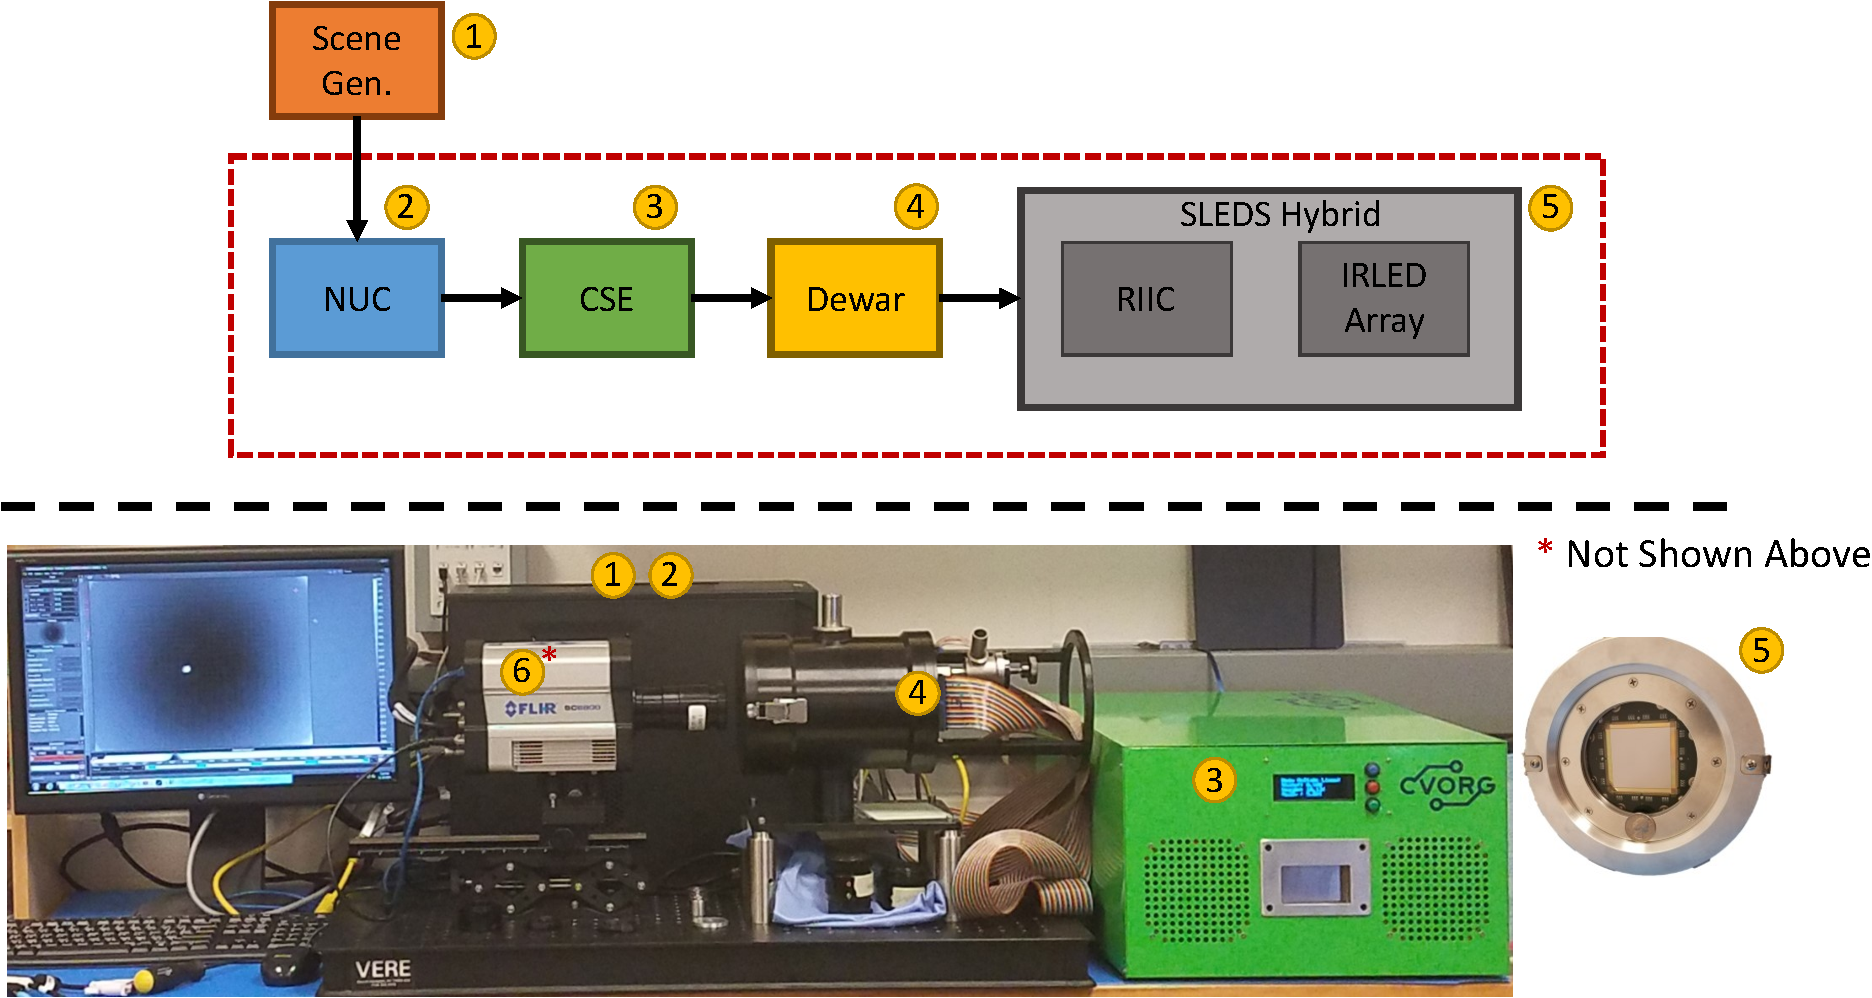
\includegraphics[width=1.0\textwidth]{fig/sleds_system.pdf}
        \caption{IRLED Scene Projector System}
        \label{fig:sleds_system}
    \end{figure}

    Figure~\ref{fig:sleds_timeline} shows the development timeline for IRLED IRSP technology. In 2008, the world's first IRLED array called the Superlattice Light Emitting Diodes (SLEDs) array was completed~\cite{AhmedEtAl2019}. This device was a hybridized combination of a 68 by 68 IRLED wafer bonded to a RIIC wafer~\cite{DasEtAl2009} providing the electronics to drive the array. Initial testing was done by hand prior the design and implementation of the overall drive system which was completed in 2011. Following this, an increased IRLED wafer of 512x512 size was fabricated in 2014~\cite{NortonEtAl2013}. The combination of the array with the drive system resulted in SLEDS (Superlattice Light Emitting Diode System), the first functioning IRLED IRSP system in the world. Further efforts culminated in two IRLED IRSPs in 2016. The first, TCSA (Two Color SLEDS Array), a 512 by 512 sized array~\cite{McGeeEtAl2015, EjzakEtAl2016, EjzakEtAl2016_2, EjzakEtAl2017, RickerEtAl2017} included support for driving the LEDs at two separate wavelength bands, denoted as 2-colors in Figure~\ref{fig:sleds_timeline}. The second, NSLEDS (N\footnote{The N originally stood for Nightglow, before the device was retargeted to Midwave-IR.} Superlattice Infrared Light Emitting Diode System), a 1024 by 1024 sized array~\cite{BenedictEtAl2017,AhmedEtAl2020} doubled the total number of pixels supported. Additionally, these systems demonstrated the beginnings of a modular IR Scene Projection (IRSP) platform~\cite{BrowningEtAl2019}. A further increase in size and efficiency occurred in 2018 with the world's first 2048 by 2048-pixel array, HDILED (High Definition Infrared LED)~\cite{BenedictEtAl2018}. A visual representation of the pixel ratios is shown in Figure~\ref{fig:tcsa_nsleds_hdiled_array_ratio}

    \begin{figure}
        \centering
        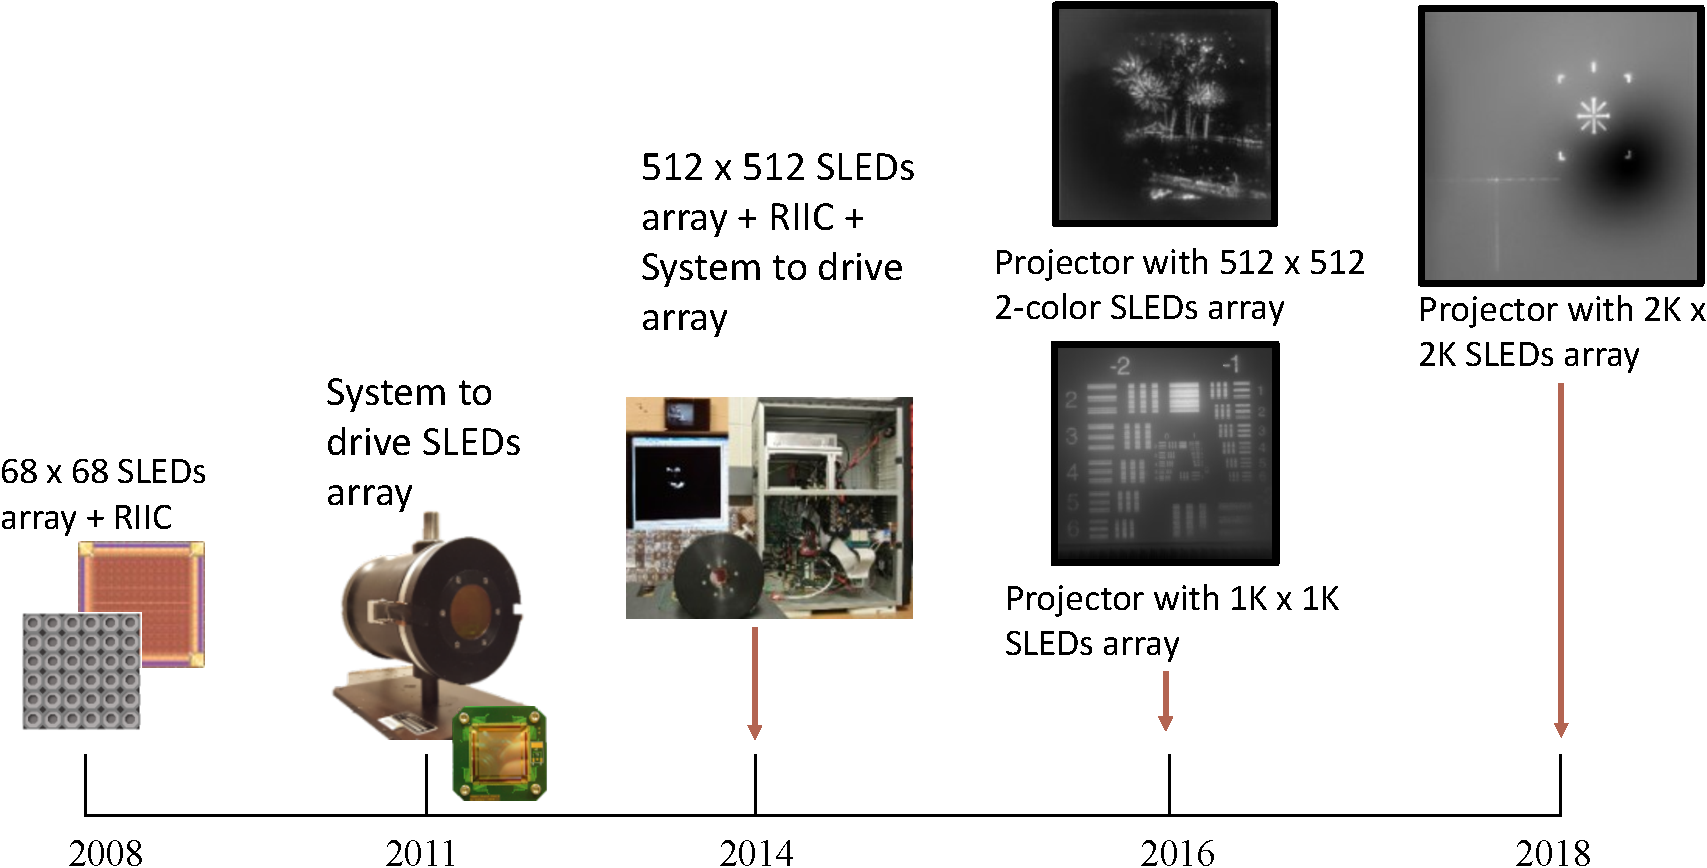
\includegraphics[width=1.0\textwidth]{fig/sleds_timeline.pdf}
        \caption{IRLED Scene Projector Technology Development Timeline Overview}
        \label{fig:sleds_timeline}
    \end{figure}

    \begin{figure}
        \centering
        %includegraphs[trim=L B R T]
        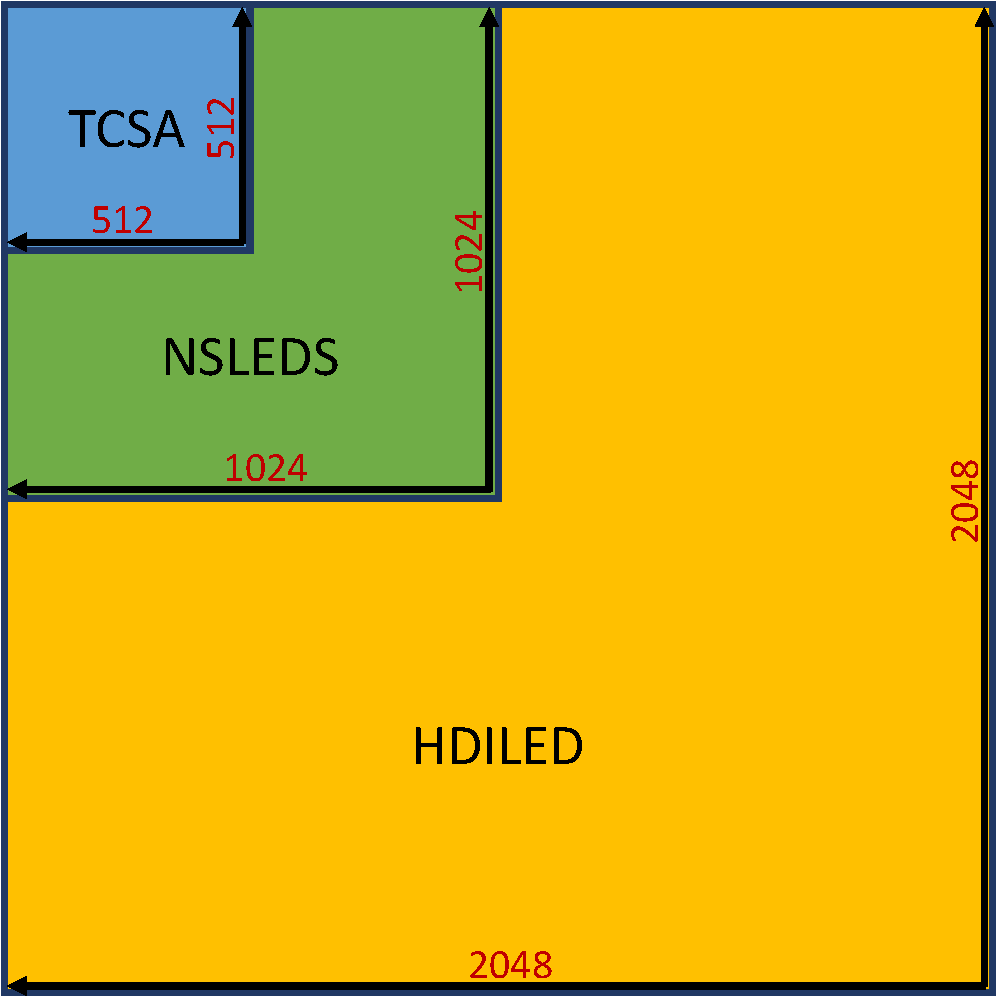
\includegraphics[width=0.5\textwidth]{fig/tcsa_nsleds_hdiled_array_ratio.pdf}
        \caption{SLEDs Array Pixel Ratios}
        \label{fig:tcsa_nsleds_hdiled_array_ratio}
    \end{figure}

    TCSA represented a novel step forward in terms of IRLED array technology. It incorporated a multiple color pixel design within a 1.3in\textsuperscript{2} package consisting of two overlayed LEDs per pixel to enable emission in multiple wave-length spectrums as well as an increase in the number of analog channels from 4 to 16 to allow for more pixels to be driven at a time. It targeted a speed of \mbox{1 kilohertz} operation. NSLEDS used the same size wafer as a TCSA, but decreased the pixel pitch from 48 to 24 microns and incorporated a single-color pixel design instead of the multiple color design of the original, these changes allowed for the pixel resolution to be doubled paving the way toward larger format IRLED IRSPs. Additionally, NSLEDS targeted \mbox{500 hertz} operation. HDILED increased the package size to 2.3in\textsuperscript{2} and doubled the resolution while utilizing a similar RIIC architecture to the prior two arrays. It targeted \mbox{250 hertz} operation. The interleaved write process of each array is discussed in detail in Chapter~\ref{sec:array_Interleaved_write_process}.

\section{IRLED Projection Process}
    Figure~\ref{fig:typical_projection} shows a typical projection process utilized within an IRLED IRSP. Each step operates at a static frame rate. A scene projector performs scene generation by utilizing a GPU typically. Following this, imagery undergoes non-uniformity correction by utilizing a NUC table created by analyzing the non-uniformity on a given array. After which, image data is reordered for sending to an array. When data is sent, a digital to analog conversion occurs for each value displayed on a projector.

    \begin{figure}
        \centering
        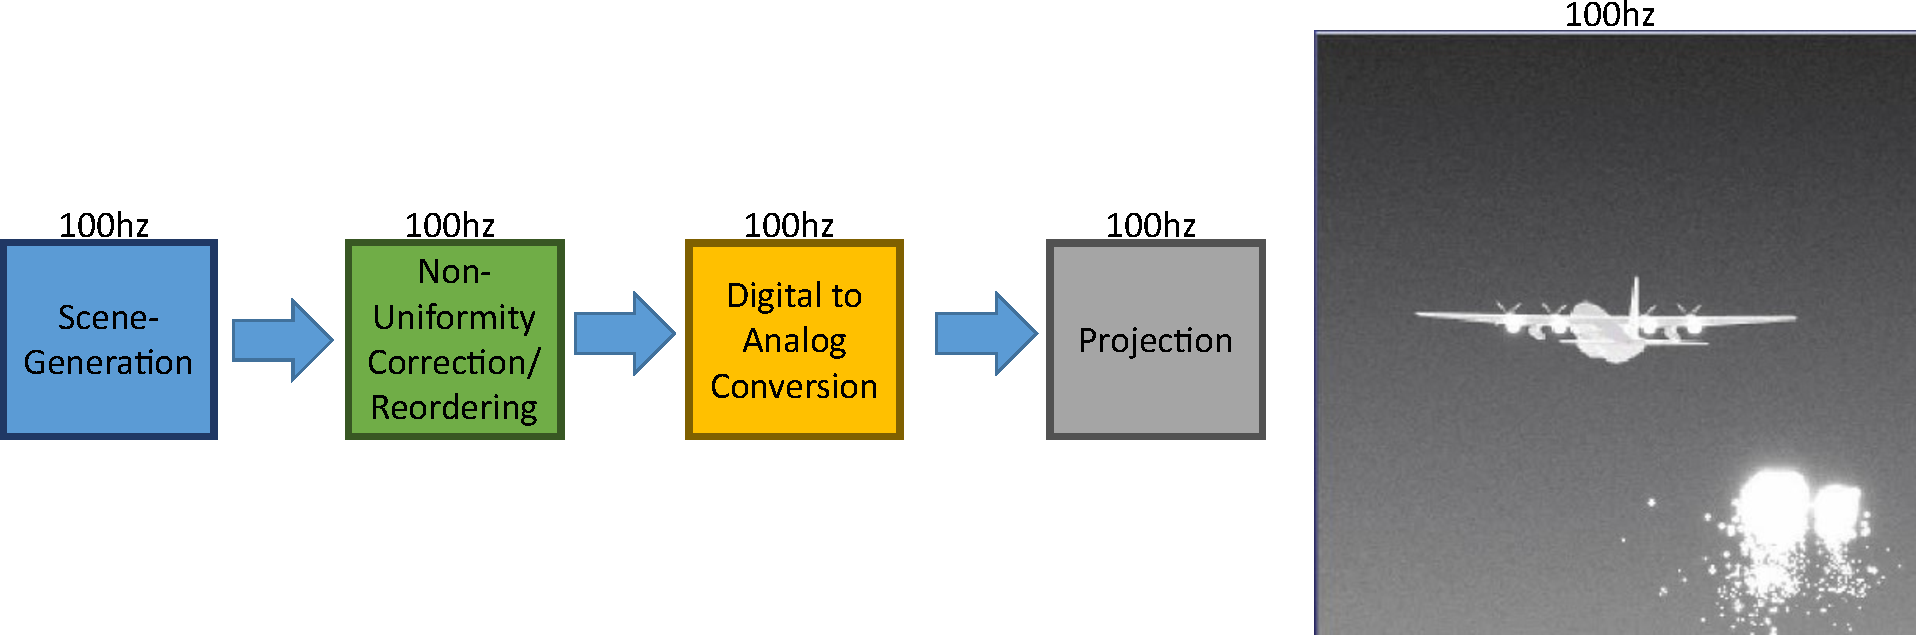
\includegraphics[width=1.0\textwidth]{fig/typical_projection_system.pdf}
        \caption{Typical IRLED Projection Process}
        \label{fig:typical_projection}
    \end{figure}

    The NUC process compensates for any physical defects that may cause non-linear variation in light emission from different diodes on a given array, thus, allowing for uniform emission across a given spectrum. There are number of different ways this linearization may be performed~\cite{BrowningEtAl2016, LandwehrEtAl2017, BarakhshanEtAl2018_2, BarakhshanEtAl2019, BarakhshanEtAl2019_2}, the details of which are beyond the scope of this work. After non-uniformity correction, imagery is converted pixel by pixel from digital to analog to drive the physical pixels at a given intensity on the array.

    The design of the digital to analogy chain of an IRLED IRSP is another important challenge as the analog bandwidth\footnote{The rise and fall time of digital-to-analog (DAC) conversion and amplification.} plays an important role in determining the maximum speed a system can operate at as well as the bit resolution\footnote{A measurement of to what degree changes to DAC inputs can produce consistent measurable light output differences.} of an array~\cite{EjzakEtAl2019}. Additionally, timing variance and potential differences in performance between analog channels needs to be analyzed and minimized through design and tuning. While outside of the scope of this work, it is worth noting that, a poorly behaving analog chain can introduce undesirable non-linear distortion in analog signaling resulting in non-linear projection ~\cite{Freeman1977, Gordon1978, ChanEtAl2008}.

    Similarly, the internal analog timings of an array's RIIC plays a critical role in this as well. One that may be considered even more crucial given that once an array is fabricated and bonded, it cannot be later modified. In contrast, a faster and more precise analog chain could be implemented at a later point in time for an existing array. Decisions made on RIIC architecture can have lasting long-term impact.

    The following chapter moves to a discussion of the central problems with display protocol technology and the proposed solution.
